% 02-results.tex — Results
% Rule: Every number comes strictly from data/tables/*.tsv. Factual descriptions only; no interpretation.

\section{Results}

\subsection{Sequencing yield and sample retention across the filtering funnel}
In the standalone upstream DADA2 demonstration dataset ($n = 41$ paired-end samples), raw demultiplexed input counts ranged from 20,545 (\texttt{FMT.0093S}) to 70,235 (\texttt{FMT.0106R}) read pairs per sample, totaling 1,832,285 input read pairs (\texttt{01\_demux\_per\_sample\_counts.tsv} and \texttt{01\_dada2\_stats.tsv}). Quality filtering retained 1,662,429 reads (90.73\% of pooled input), denoising retained 1,654,313 reads (90.29\%), paired-end merging retained 1,608,758 reads (87.80\%), and chimera removal yielded 1,535,600 non-chimeric reads (83.81\% of pooled input) distributed across 660 ASVs (Figure~\ref{fig:filtering}B; Table~\ref{tab:funnel}). At the individual sample level, the percentage of input reads retained as non-chimeric sequences ranged from 71.18\% (\texttt{FMT.0107B}; 17,695 of 24,858 reads) to 92.40\% (\texttt{FMT.0106M}; 48,097 of 52,054 reads), with a mean per-sample retention rate of 84.22\%.

In the downstream clinical reanalysis starting from the full repository table of 12,546 samples, 17,865 ASVs, and 550,243,459 reads (\texttt{00\_filtering\_funnel.tsv}), restricting to samples with a defined randomized group (\texttt{autoFmtGroup IS NOT NULL}) retained 556 samples (4.43\% of initial samples), 4,256 ASVs, and 27,997,124 reads (Figure~\ref{fig:filtering}A; Table~\ref{tab:funnel}). Constraining the longitudinal window to days $-10$ through $+70$ relative to allo-HCT reduced the dataset to 406 samples, 3,680 ASVs, and 23,069,077 reads. Removing singleton ASVs present in only one sample (\texttt{--p-min-samples 2}) eliminated 1,222 features while retaining all 406 samples, 2,458 ASVs, and 22,972,681 reads. Excluding features without a phylum assignment or classified as chloroplast or mitochondrial sequences removed an additional 33 ASVs, leaving 406 samples, 2,425 ASVs, and 22,909,139 reads. Finally, enforcing a minimum sequencing depth of 10,000 reads per sample (\texttt{--p-min-frequency 10000}) excluded 50 samples (12.32\% of the 406 in-window samples) and 3 ASVs, resulting in a final analytical cohort of 356 samples, 2,422 ASVs, and 22,692,526 reads across 24 patients (Table~\ref{tab:funnel}).

\begin{table}[t]
\centering
\footnotesize
\setlength{\tabcolsep}{3pt}
\caption{Sample, feature (ASV), and sequencing read counts across the upstream DADA2 demonstration and the five-step downstream filtering funnel (\texttt{00\_filtering\_funnel.tsv}).}
\label{tab:funnel}
\begin{tabular}{llrrr}
\toprule
Stage & Filtering criterion & Samples ($n$) & ASVs ($n$) & Total reads \\
\midrule
\texttt{upstream\_dada2} & Standalone 41-sample DADA2 denoising demo & 41 & 660 & 1,535,600 \\
\midrule
\texttt{0\_raw} & Full FigShare repository table (downstream start) & 12,546 & 17,865 & 550,243,459 \\
\texttt{1\_trial\_cohort} & \texttt{autoFmtGroup IS NOT NULL} & 556 & 4,256 & 27,997,124 \\
\texttt{2\_time\_window} & \texttt{DayRelativeToNearestHCT} in $[-10, 70]$ & 406 & 3,680 & 23,069,077 \\
\texttt{3\_prevalence} & Present in $\ge 2$ samples (\texttt{--p-min-samples 2}) & 406 & 2,458 & 22,972,681 \\
\texttt{4\_taxonomy} & Retain \texttt{p\_\_}; exclude Chloroplast/Mitochondria & 406 & 2,425 & 22,909,139 \\
\texttt{5\_depth} & Depth $\ge 10,000$ reads (\texttt{--p-min-frequency 10000}) & 356 & 2,422 & 22,692,526 \\
\bottomrule
\end{tabular}
\end{table}

\begin{figure}[t]
\centering
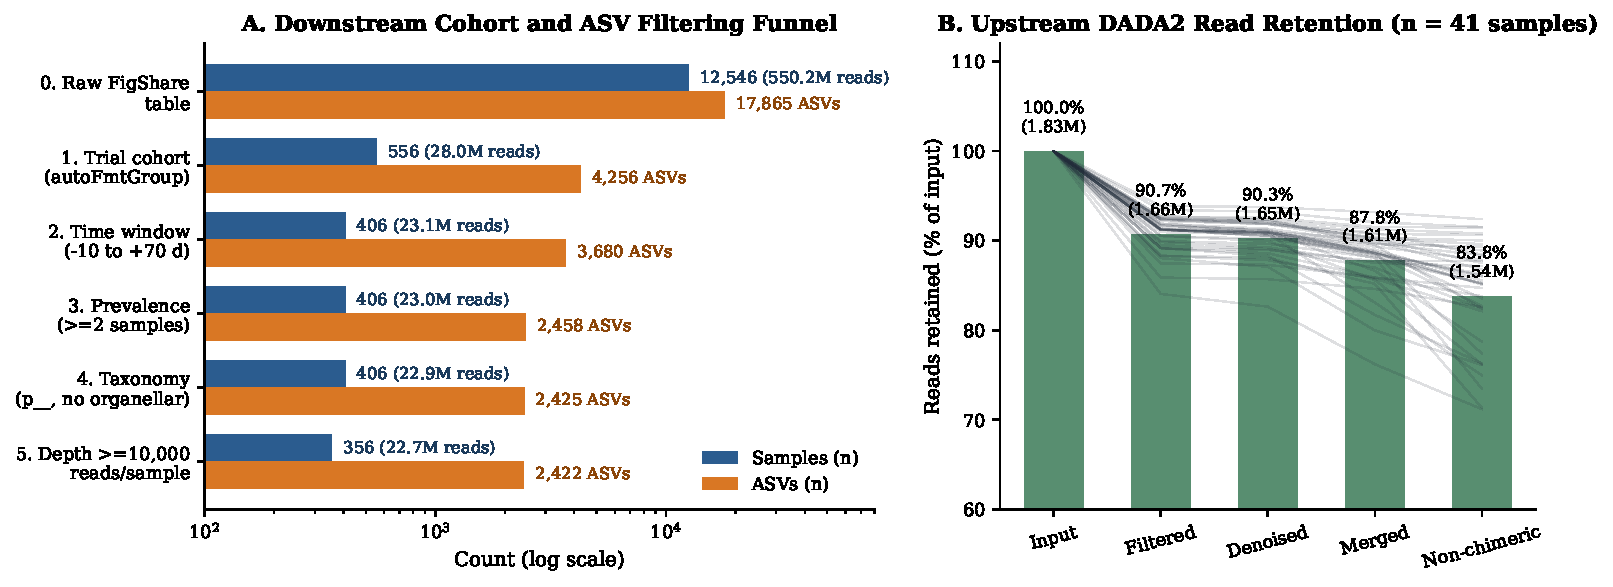
\includegraphics[width=\linewidth]{fig1_filtering_and_qc.pdf}
\caption{Cohort filtering funnel and upstream denoising retention. (\textbf{A}) Sample and ASV counts (log scale) and total sequencing reads across the six stages of the downstream filtering funnel (\texttt{00\_filtering\_funnel.tsv}). (\textbf{B}) Percentage and total count of input reads retained across sequential DADA2 denoising steps for the 41 upstream demonstration samples (\texttt{01\_dada2\_stats.tsv}); gray lines trace individual sample retention trajectories.}
\label{fig:filtering}
\end{figure}

\subsection{Cross-sectional alpha diversity comparisons and beta diversity ordination}
Pairwise Kruskal-Wallis tests on rarefied ASV richness (\texttt{observed\_features} at 10,000 reads/sample; $n = 356$ samples) across clinical and temporal groupings are summarized in Figure~\ref{fig:diversity}A. Across time categories relative to allo-HCT (\texttt{02\_kruskal\_categorical-time-relative-to-hct.tsv}), significant differences in observed ASVs were detected between \texttt{post} ($n = 225$) and \texttt{pre} ($n = 78$) samples ($H = 70.58$, $p = 4.42 \times 10^{-17}$, $q = 1.33 \times 10^{-16}$), between \texttt{peri} ($n = 53$) and \texttt{pre} ($n = 78$) samples ($H = 20.38$, $p = 6.36 \times 10^{-6}$, $q = 9.54 \times 10^{-6}$), and between \texttt{peri} ($n = 53$) and \texttt{post} ($n = 225$) samples ($H = 8.51$, $p = 0.00354$, $q = 0.00354$). When stratified by time categories relative to FMT (\texttt{02\_kruskal\_categorical-time-relative-to-fmt.tsv}), richness differed between \texttt{peri} ($n = 27$) and \texttt{post} ($n = 41$) samples ($H = 10.42$, $p = 0.00125$, $q = 0.00374$) and between \texttt{peri} ($n = 27$) and \texttt{pre} ($n = 288$) samples ($H = 5.87$, $p = 0.0154$, $q = 0.0231$), whereas no significant difference was observed between \texttt{post} ($n = 41$) and \texttt{pre} ($n = 288$) samples ($H = 1.58$, $p = 0.208$, $q = 0.208$).

In contrast, when all 356 samples were pooled across time points to compare the randomized intervention arms (\texttt{02\_kruskal\_autoFmtGroup.tsv}), observed ASV richness did not differ significantly between the control group ($n = 150$ samples) and the auto-FMT treatment group ($n = 206$ samples; $H = 1.29$, $p = 0.256$, $q = 0.256$; Figure~\ref{fig:diversity}A). Among clinical covariates, pairwise comparisons by stool consistency (\texttt{02\_kruskal\_Consistency.tsv}; $n = 355$ annotated samples) showed significant differences between \texttt{formed} ($n = 97$) and \texttt{semi-formed} ($n = 115$) stools ($H = 8.26$, $p = 0.00405$, $q = 0.0121$) and between \texttt{formed} ($n = 97$) and \texttt{liquid} ($n = 143$) stools ($H = 5.55$, $p = 0.0185$, $q = 0.0277$), but not between \texttt{liquid} and \texttt{semi-formed} stools ($H = 0.44$, $p = 0.507$, $q = 0.507$). Across stem cell graft sources (\texttt{02\_kruskal\_HCTSource.tsv}), significant differences were observed for unmodified bone marrow (\texttt{BM\_unmodified}, $n = 67$) versus unmodified peripheral blood stem cells (\texttt{PBSC\_unmodified}, $n = 128$; $H = 21.20$, $p = 4.14 \times 10^{-6}$, $q = 2.49 \times 10^{-5}$), \texttt{PBSC\_unmodified} ($n = 128$) versus T-cell depleted grafts (\texttt{TCD}, $n = 129$; $H = 18.86$, $p = 1.41 \times 10^{-5}$, $q = 4.22 \times 10^{-5}$), \texttt{BM\_unmodified} ($n = 67$) versus umbilical cord blood (\texttt{cord}, $n = 32$; $H = 10.30$, $p = 0.00133$, $q = 0.00266$), and \texttt{TCD} ($n = 129$) versus \texttt{cord} ($n = 32$; $H = 7.85$, $p = 0.00507$, $q = 0.00761$), whereas \texttt{BM\_unmodified} versus \texttt{TCD} ($H = 2.09$, $p = 0.149$, $q = 0.178$) and \texttt{PBSC\_unmodified} versus \texttt{cord} ($H = 0.013$, $p = 0.908$, $q = 0.908$) were not statistically significant.

In beta diversity PCoA ordinations (\texttt{05\_pcoa\_proportion\_explained.tsv}; Figure~\ref{fig:diversity}B), weighted UniFrac captured the highest proportion of variance along the first three principal coordinates (PC1 = 31.61\%, PC2 = 11.55\%, PC3 = 11.48\%; cumulative 54.64\%), followed by unweighted UniFrac (PC1 = 20.42\%, PC2 = 6.25\%, PC3 = 4.43\%; cumulative 31.10\%), Bray-Curtis dissimilarity (PC1 = 13.90\%, PC2 = 10.65\%, PC3 = 5.64\%; cumulative 30.19\%), and Jaccard distance (PC1 = 6.86\%, PC2 = 3.40\%, PC3 = 2.79\%; cumulative 13.05\%).

\begin{figure}[t]
\centering
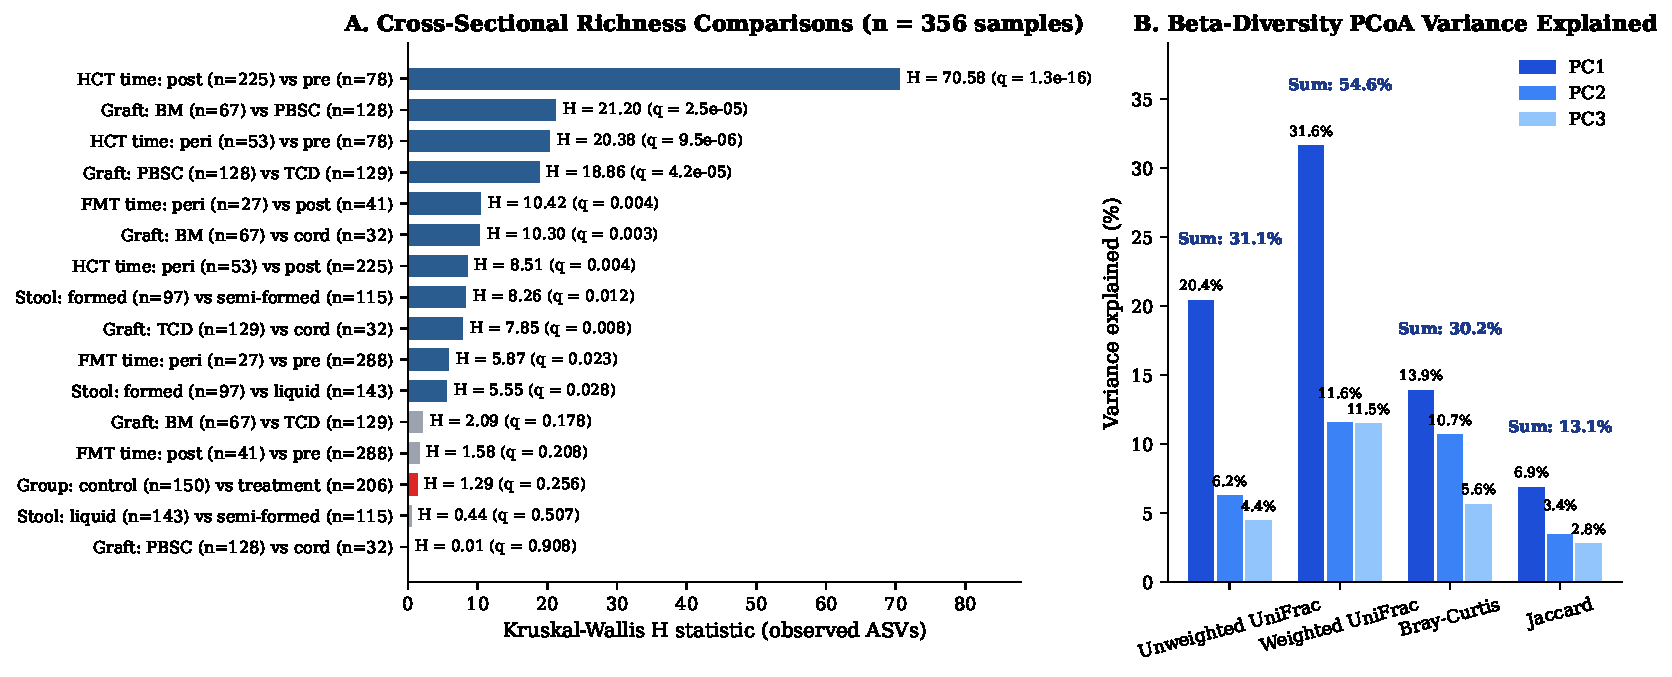
\includegraphics[width=\linewidth]{fig2_diversity_and_pcoa.pdf}
\caption{Cross-sectional alpha diversity comparisons and beta diversity ordination variance explained. (\textbf{A}) Pairwise Kruskal-Wallis $H$ statistics and Benjamini-Hochberg FDR-adjusted $q$-values for observed ASVs across temporal and clinical metadata groupings (\texttt{02\_kruskal\_*.tsv}); blue bars denote $q < 0.05$, gray bars denote $q \ge 0.05$, and the red bar highlights the pooled comparison between control and auto-FMT treatment groups ($H = 1.29$, $q = 0.256$). (\textbf{B}) Percentage of variance explained by the first three principal coordinates (PC1--PC3) across four beta diversity distance metrics (\texttt{05\_pcoa\_proportion\_explained.tsv}).}
\label{fig:diversity}
\end{figure}

\subsection{Longitudinal trajectory of microbial richness via linear mixed-effects modeling}
The linear mixed-effects (LME) model fit via REML evaluated \texttt{observed\_features} across 356 observations nested within 24 patients (2 to 34 observations per patient, mean 14.8; residual scale = 1,757.408, log-likelihood = $-1,840.587$; \texttt{03\_lme\_model\_summary.tsv}). Notably, the model summary recorded that the optimization algorithm did not converge (\texttt{Converged: No}).

Fixed- and random-effect parameter estimates from \texttt{03\_lme\_model\_results.tsv} are presented in Table~\ref{tab:lme} and Figure~\ref{fig:lme}. At day 0 relative to FMT, the baseline intercept for the control group was 65.687 observed ASVs ($\text{SE} = 6.696$, $z = 9.811$, $p < 0.001$, 95\% CI $[52.564, 78.810]$), and the main effect for the auto-FMT treatment group at day 0 was $+2.962$ ASVs ($\text{SE} = 8.849$, $z = 0.335$, $p = 0.738$, 95\% CI $[-14.381, 20.306]$). Across time (\texttt{day-relative-to-fmt}), the control group exhibited a statistically significant linear decline of $-0.859$ observed ASVs per day ($\text{SE} = 0.172$, $z = -5.003$, $p < 0.001$, 95\% CI $[-1.196, -0.523]$). The group-by-time interaction term (\texttt{day-relative-to-fmt:autoFmtGroup[T.treatment]}) was $+0.560$ observed ASVs per day ($\text{SE} = 0.232$, $z = 2.409$, $p = 0.016$, 95\% CI $[0.104, 1.015]$), corresponding to an implied net slope of $-0.299$ observed ASVs per day ($-0.859 + 0.560$) in the auto-FMT treatment group (Figure~\ref{fig:lme}A--B). The between-patient random intercept variance (\texttt{Group Var}) was 197.005 ($\text{SE} = 2.058$).

\begin{table}[t]
\centering
\footnotesize
\setlength{\tabcolsep}{3pt}
\caption{Linear mixed-effects (LME) model parameter estimates for \texttt{observed\_features} across 356 samples from 24 patients (\texttt{03\_lme\_model\_results.tsv} and \texttt{03\_lme\_model\_summary.tsv}; REML scale = 1,757.408, log-likelihood = $-1,840.587$, \texttt{Converged: No}).}
\label{tab:lme}
\begin{tabular}{lrrrrrr}
\toprule
Model term & Coef. & Std.\ Err. & $z$ & $P > |z|$ & 95\% CI low & 95\% CI high \\
\midrule
Intercept (Control at day 0) & 65.687 & 6.696 & 9.811 & $< 0.001$ & 52.564 & 78.810 \\
\texttt{autoFmtGroup[T.treatment]} & 2.962 & 8.849 & 0.335 & 0.738 & $-14.381$ & 20.306 \\
\texttt{day-relative-to-fmt} (Control) & $-0.859$ & 0.172 & $-5.003$ & $< 0.001$ & $-1.196$ & $-0.523$ \\
\texttt{day-relative-to-fmt:treatment} & 0.560 & 0.232 & 2.409 & 0.016 & 0.104 & 1.015 \\
\midrule
Patient random intercept (\texttt{Group Var}) & 197.005 & 2.058 & --- & --- & --- & --- \\
\bottomrule
\end{tabular}
\end{table}

\begin{figure}[t]
\centering
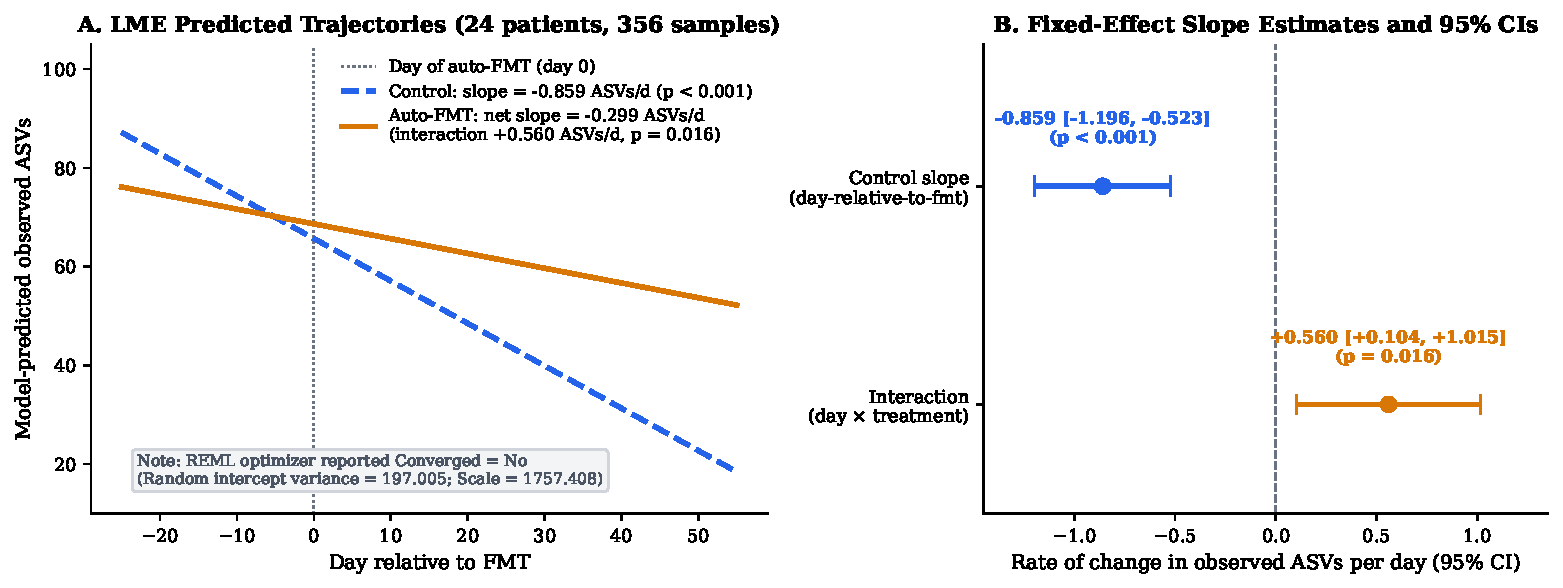
\includegraphics[width=\linewidth]{fig3_lme_trajectories.pdf}
\caption{Longitudinal linear mixed-effects (LME) model of observed ASV richness relative to FMT day. (\textbf{A}) Model-predicted linear trajectories of \texttt{observed\_features} for the control group (dashed blue line; slope $= -0.859$ ASVs/day) and the auto-FMT treatment group (solid orange line; implied net slope $= -0.299$ ASVs/day). (\textbf{B}) Point estimates and 95\% confidence intervals for the daily rate of change in the control group and the group-by-time interaction term (\texttt{03\_lme\_model\_results.tsv}).}
\label{fig:lme}
\end{figure}

\subsection{Temporal succession of microbial taxa predicted by random forest regression}
In the longitudinal feature volatility analysis (\texttt{04\_rf\_accuracy.tsv}), the random forest regressor trained on conditionally filtered genus-level relative frequencies predicted \texttt{week-relative-to-hct} with a mean squared error (MSE) of 4.249, Pearson correlation $r = 0.565$, coefficient of determination $R^2 = 0.319$, and $p = 2.37 \times 10^{-7}$ (linear fit slope $= 0.304$, standard error $= 0.053$, intercept $= 0.991$).

Twenty genus-level features met the prevalence ($\ge 10\%$ of samples) and abundance ($\ge 1\%$) thresholds and contributed to the random forest model (\texttt{04\_rf\_feature\_importance.tsv}; Figure~\ref{fig:rf}). The four highest-ranking features accounted for 40.92\% of total model importance: unclassified \textit{Enterococcaceae} (importance $= 0.124$), \textit{Clostridium} (family \textit{Clostridiaceae}; $0.109$), \textit{Enterococcaceae} genus \textit{Incertae Sedis} ($0.089$), and unclassified \textit{Lachnospiraceae} ($0.087$). Combined, the two \textit{Enterococcaceae} features accounted for 21.30\% of total importance, while the three \textit{Lachnospiraceae} features---unclassified \textit{Lachnospiraceae} ($0.087$), \textit{Murimonas} ($0.036$), and \textit{Sellimonas} ($0.033$)---accounted for 15.68\%. Additional features with importance scores above 0.030 included unclassified \textit{Actinobacteria} ($0.077$), unclassified \textit{Erysipelotrichaceae} ($0.061$), \textit{Tannockella} ($0.054$), unclassified \textit{Lactobacillaceae} ($0.047$), \textit{Streptococcus} ($0.046$), unclassified \textit{Bifidobacteriaceae} ($0.037$), \textit{Staphylococcus} ($0.035$), and \textit{Asaccharospora} ($0.035$), whereas \textit{Lactococcus} ($0.029$), unclassified \textit{Ruminococcaceae} ($0.026$), \textit{Akkermansia} ($0.023$), \textit{Veillonella} ($0.018$), \textit{Longicatena} ($0.017$), and \textit{Escherichia-Shigella} ($0.015$) each contributed less than 0.030 (Figure~\ref{fig:rf}).

\begin{figure}[t]
\centering
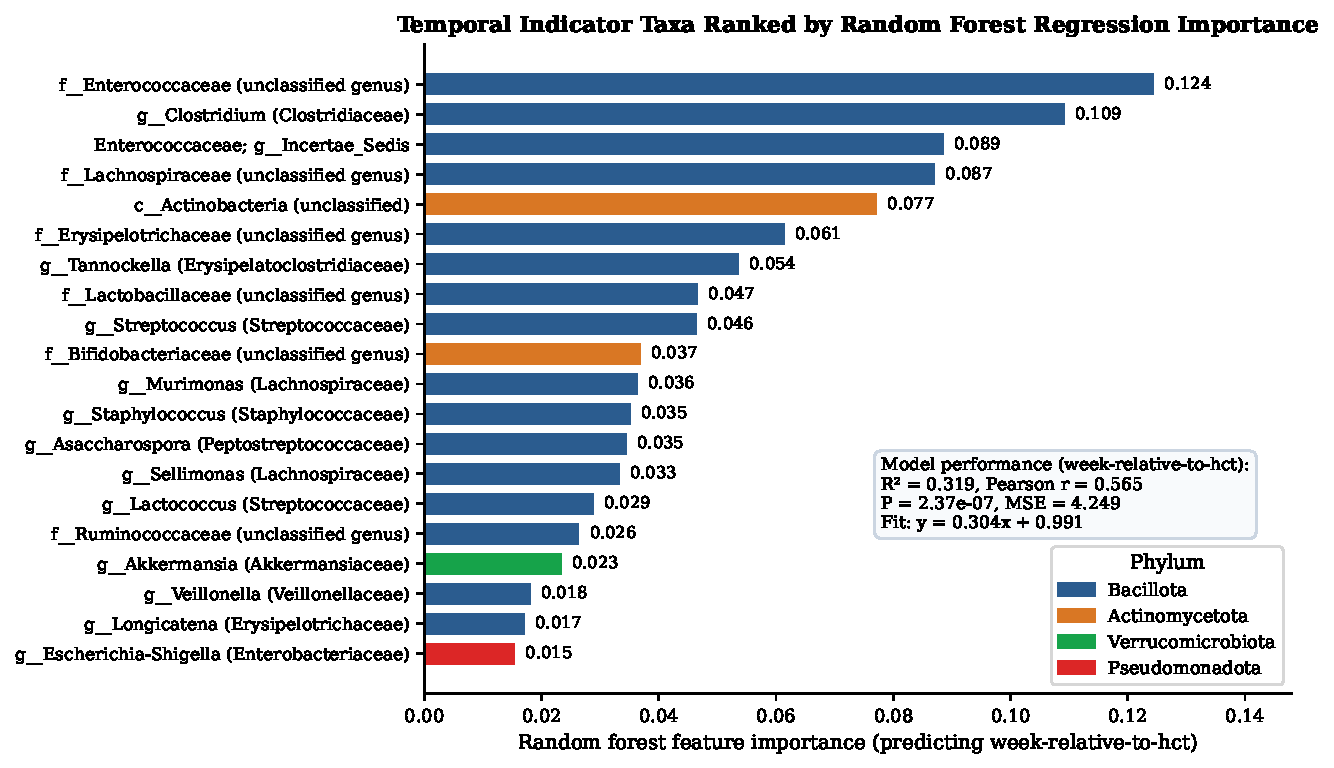
\includegraphics[width=0.92\linewidth]{fig4_rf_feature_importance.pdf}
\caption{Normalized feature importance scores of the 20 genus-level taxa retained in the random forest regression model predicting \texttt{week-relative-to-hct} (\texttt{04\_rf\_feature\_importance.tsv} and \texttt{04\_rf\_accuracy.tsv}). Bars are colored by bacterial phylum.}
\label{fig:rf}
\end{figure}
